\documentclass{standalone} % (c) Jan Suchanek 2023  cc by
\usepackage{tikz}
\usepackage{xcolor}

\usetikzlibrary{decorations.text}
\begin{document}
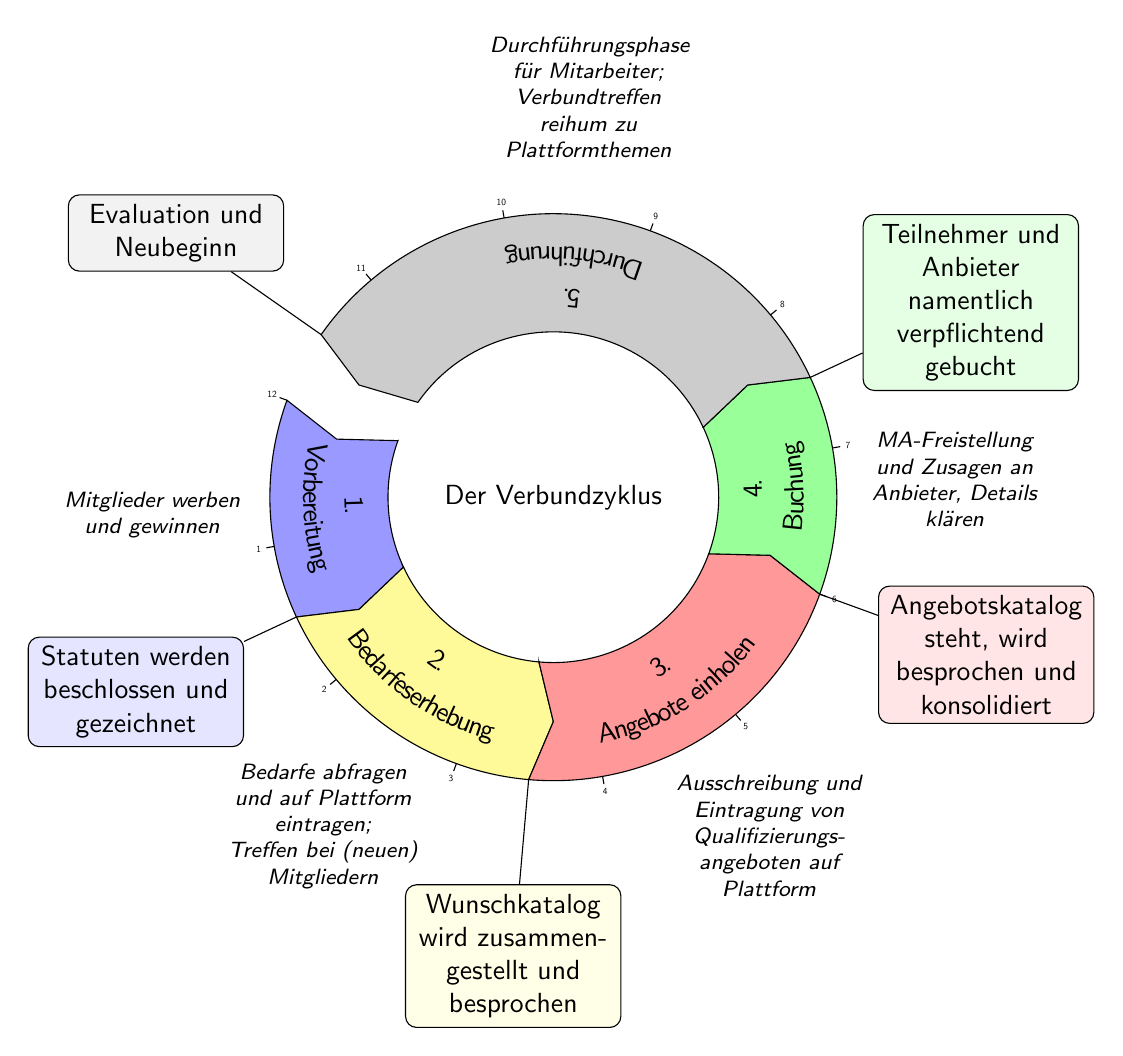
\begin{tikzpicture} % rotate to suit your needs
[rotate=160,every node/.style={font=\sffamily}]

\def\myraise{1.5} % ring thickness
\def\myradius{3.6} % inner radius

\def\anfang{0} % variable: starting points of task
\def\mitte{0} % variable: mid points of task
\def\ende{0} % variable: end points of task

\def\schritte{12} % units in which duration is measuerd: use 52 for a weekly cylce, 12 for months, 12 or 24 for hours etc.

\def\zentrumtext{Der Verbundzyklus} % to be written in the center of the ring (inside a \parbox)

\pgfmathparse{360/\schritte}
\xdef\inkrement{\pgfmathresult} % angle per unit

\foreach \i in {1,...,\schritte} % draws a counter-clockwise-"clock" for orientation
{
\draw (\i*\inkrement:\myradius) -- (\i*\inkrement:\myradius+0.1);
\node at (\i*\inkrement:\myradius+0.2) {\resizebox{!}{0.5ex}{\i}};
}

\node % write centertext into the middle. Could also be an image etc.
at (0,0) {
\parbox{\myradius cm}{
\centering
\zentrumtext\\
}
};

%% now the actual ring. The foreach list includes
% \dauer - duration of the taskt
% \task - to be written on the ring
% \mittetext - to be written outside the ring in the middle of the task
% \ergebnis - milestone or result, written in a frame at the end of task
% \farbe - the color of task an milestone
% Note: last entry must end with %
\foreach [count=\ii] \dauer/\task/\mittetext/\ergebnis/\farbe in {
1.5/Vorbereitung/Mitglieder werben und gewinnen/Statuten werden beschlossen und gezeichnet/blue,
2/Bedarfeserhebung/Bedarfe abfragen und auf Plattform eintragen;\\ Treffen bei (neuen) Mitgliedern/Wunschkatalog wird zusammen\-gestellt und besprochen/yellow,
2.5/Angebote einholen/Ausschreibung und Eintragung von Qualifizierungs\-angeboten auf Plattform/Angebots\-katalog steht{,} wird besprochen und konsolidiert/red,
1.5/Buchung/MA-Freistellung und Zusagen an Anbieter{,} Details klären/Teilnehmer und Anbieter namentlich verpflichtend gebucht/green,
4/Durchf{ü}hrung/Durchf{ü}hrungsphase für Mitarbeiter; Verbundtreffen reihum zu Plattformthemen/Evaluation und Neubeginn/gray%
}{

\pgfmathparse{\anfang+\dauer} % calculates end of task
\xdef\ende{\pgfmathresult} %

\filldraw[\farbe!40,draw=black] % draw the bent arrow
(\ende*\inkrement:\myradius-\myraise) arc (\ende*\inkrement:\anfang*\inkrement:\myradius-\myraise)
-- (\anfang*\inkrement:\myradius-\myraise)
-- (\anfang*\inkrement+5:\myradius-0.5*\myraise)
-- (\anfang*\inkrement:\myradius) arc (\anfang*\inkrement:(\ende*\inkrement):\myradius)
-- (\ende*\inkrement+5:\myradius-0.5*\myraise)
-- cycle;

\draw % put text inside the arrow
[decoration={
text along path,
text={|\sffamily|\ii.},
text align={center},
raise=18*\myraise},decorate]
(\anfang*\inkrement:\myradius) arc (\anfang*\inkrement:\ende*\inkrement:\myradius);
\draw
[decoration={
text along path,
text={|\sffamily|\task},
text align={center},
raise=8*\myraise},decorate]
(\anfang*\inkrement:\myradius) arc (\anfang*\inkrement:\ende*\inkrement:\myradius);

\pgfmathparse{\anfang+\dauer/2} % calculate middle of task
\xdef\mitte{\pgfmathresult}

\node % put the explanatory text outside the arrow at middle of task
(mitte) at (\mitte*\inkrement:\myradius+1*\myraise) {
\parbox{2.5cm}{
\centering\footnotesize
\textit{\mittetext}
}
};

\node % draw colored box with the result at end of task
[draw, rounded corners,fill=\farbe!10] (ende) at (\ende*\inkrement:\myradius+1.5*\myraise) {
\parbox{2.5cm}{
\centering
\ergebnis
}
};

\draw % connect said box to the end of task
(\ende*\inkrement:\myradius) -- (ende);

\pgfmathparse{\anfang+\dauer} % set \anfang to the end of current task for next task
\xdef\anfang{\pgfmathresult}
}
\end{tikzpicture}
\end{document}